\chapter{Background on DEVS Modeling Formalism}
\label{Chapter:DEVS}

Discrete Event System Specification (DEVS) is a modeling and analysis formalism for discrete event systems \cite{Zeigler84}. Modular and hierarchical moduling views are two important aspects in DEVS formalism. Modularity is achieved by input and output events whereas hierarchical aspect is realized by the coupling operation.

A DEVS system is formed of states, input and output events, a notion of time, and functions that describe how the system evolves with respect to input and output events.

There are two types of DEVS models. Atomic DEVS models enable a system to be modeled modularly by first creating models by simple fundamental dynamic behaviors. Coupled DEVS models enables the definition of the system hierarchically by coupling the atomic models to create a complete system specification. Mathematical definitions of those models will be given in the next sections.

\section{Atomic DEVS Models}

\begin{figure}
 \centering
 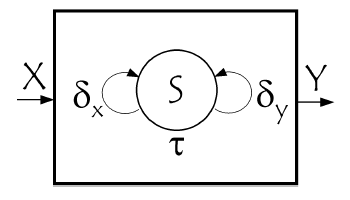
\includegraphics[width=0.75\textwidth]{figures/atomicdevs.png}
 % atomicdevs.png: 143406760x143406768 pixel, 0dpi, infxinf cm, bb=
 \caption{Symmetric Structure of Atomic DEVS}
 \label{fig:atomicdevs}
\end{figure}

An atomic DEVS is a 7-tuple structure $A = < X, Y, S, s_{0}, \tau, \delta_{x}, \delta{y} >$ \cite{Devspp} where

\begin{itemize}
 \item $X$ is a set of \textit{input events}.
 \item $Y$ is a set of \textit{output events}.
 \item $S$ is a set of \textit{states}.
 \item $s_{0} \in S$ is the initial state.
 \item $\tau ; S \rightarrow T$ is the \textit{time advance function} where $T = [0,\infty]$ is the set of non-negative real numbers plus the transfinite number, infinity. This function is used to determine the lifespan of a state.
 \item $\delta_{x} : P \times X \rightarrow S \times {0,1}$ is the \textit{input transition function} where $P = \left\{(s, t_{s}, t_{e}) | s \in S, t_{s} \in T, t_{e} \ in [0, t_{s}]\right\}$
\end{itemize}

There are two types of transitions in an atomic DEVS model: external and internal transitions. These transitions are the only ways a model can change its state. Internal transitions are time-based. That is, a transition occurs when the elapsed time reaches to the lifetime of the state which is defined by $\tau(s)$. An internal transition not only causes a state change but may also generate an output event. External transitions are event-based. That is, a transition occurs when an input event arrives. An input event causes a state change when the conditions given by $\delta_{x}$ is satisfied. External transitions are instantaneous and only trigger state change and do not generate an output event.

Figure \ref{fig:atomicdevs} demonstrates an atomic DEVS model. 


\section{Coupled DEVS Models}

A coupled DEVS is also a 7-tuple structure \cite{Devspp} $N = < X, Y, D, \left\{M_{i}\right\}, EIC, ITC, EOC >$ where

\begin{itemize}
 \item $X$ is a set of input events
 \item $Y$ is a set of output events
 \item $D$ is a set of names of subcomponents
 \item $\left\{M_{i}\right\}$ is a set of DEVS models where $i \in D$. $M_{i}$ can be either atomic DEVS model or a coupled DEVS model
 \item $EIC \subseteq X \times \underset{i \in D}{\cup} X_{i}$ is a set of external input couplings where $X_{i}$ is the set of input events of $M{i}$.
 \item $ITC \subseteq \underset{i \in D}{\cup}Y_{i} \times \underset{i \in D}{\cup} X_{i}$ is a set of internal couplings where $Y_{i}$ is the set of output events of $M_{i}$.
 \item $EOC \subseteq \underset{i \in D}{\cup}Y_{i} \times Y$ is a set of external couplings.
\end{itemize}

A coupled DEVS model defines the subsystems that are contained by the model and how there are connected to each other. Coupled DEVS models realize the modular and hierarchical aspect of the DEVS formalism by enabling a system designer to build a larger system by designing and connecting simpler subsystems. Although it is not impossible to create a complete system only with atomic models, it is very tedious and error prone. Coupled DEVS model eliminates this complexity and lets subsystems be composed together and connected to each other enabling a better system specification.

Since the resulting DEVS model is modular and hierarchical, events generated within a subsystems can propoage through other parts of the subsystem horizantally, or through other subsystems vertically within the hieararchy of the system through well defined interfaces. 

\section{Summary}

DEVS formalism  provides the means to describe discrete event systems and provides constructs like time, events, states and transitions as well as composition of models. In this research, DEVS was chosen to be used to model parts of a distributed data acquistion system. Event-based nature of the data acquistion system made DEVS the proper tool to model its middleware and applications using the DEVS modeling formalism. Open DEVS simulation framework \cite{Devspp} provides suitable ground work to model applications as DEVS models and simulate the complete system.
